% move all configuration stuff into one file so we can focus on the content
\documentclass[aspectratio=169,hyperref={pdfpagelabels=false,colorlinks=true,linkcolor=white,urlcolor=blue},t]{beamer}

%%%%%%%%%%%%%%%%%%%%%%%%%%%%%%%%%%%%%%%%%%%%%%%%%%%%%%%%%%%%%%%%%%%%%%%%%%%%%%%%%%
%%%%%%%%%%%%%%%%%%%%%%%%%%%%%%%%%%%%%%%%%%%%%%%%%%%%%%%%%%%%%%%%%%%%%%%%%%%%%%%%%%
% packages
\usepackage{pict2e}
\usepackage{epic}
\usepackage{amsmath,amsfonts,amssymb}
\usepackage{units}
\usepackage{fancybox}
\usepackage[absolute,overlay]{textpos} 
\usepackage{media9} % avi2flv: "C:\Program Files\ffmpeg\bin\ffmpeg.exe" -i TuneFreqFilterbank.avi -b 600k -s 441x324 -r 15 -acodec copy TuneFreqFilterbank.flv
\usepackage{animate}
\usepackage{gensymb}
\usepackage{multirow}
\usepackage{silence}
\usepackage[backend=bibtex,style=ieee]{biblatex}
\AtEveryCitekey{\iffootnote{\tiny}{}}
\addbibresource{references}

%%%%%%%%%%%%%%%%%%%%%%%%%%%%%%%%%%%%%%%%%%%%%%%%%%%%%%%%%%%%%%%%%%%%%%%%%%%%%%%%%%
%%%%%%%%%%%%%%%%%%%%%%%%%%%%%%%%%%%%%%%%%%%%%%%%%%%%%%%%%%%%%%%%%%%%%%%%%%%%%%%%%%
% relative paths
\graphicspath{{graph/}}


%%%%%%%%%%%%%%%%%%%%%%%%%%%%%%%%%%%%%%%%%%%%%%%%%%%%%%%%%%%%%%%%%%%%%%%%%%%%%%%%%%
%%%%%%%%%%%%%%%%%%%%%%%%%%%%%%%%%%%%%%%%%%%%%%%%%%%%%%%%%%%%%%%%%%%%%%%%%%%%%%%%%%
% units
\setlength{\unitlength}{1mm}

%%%%%%%%%%%%%%%%%%%%%%%%%%%%%%%%%%%%%%%%%%%%%%%%%%%%%%%%%%%%%%%%%%%%%%%%%%%%%%%%%%
%%%%%%%%%%%%%%%%%%%%%%%%%%%%%%%%%%%%%%%%%%%%%%%%%%%%%%%%%%%%%%%%%%%%%%%%%%%%%%%%%%
% theme & layout
\usetheme{Frankfurt}
\beamertemplatenavigationsymbolsempty
%\setbeamertemplate{frametitle}[smoothbars theme]
\setbeamertemplate{frametitle}
{
    \begin{beamercolorbox}[ht=1.8em,wd=\paperwidth]{frametitle}
        \vspace{-.1em}%
        \hspace{.2em}{\strut\insertframetitle\strut}
        
        \hspace{.2em}\small\strut\insertframesubtitle\strut
        %\hfill
        %
\includegraphics[height=.8cm,keepaspectratio]{CenterMusicTechnology-solid-2lines-white-CoAtag}
        
    \end{beamercolorbox}
    \begin{textblock*}{100mm}(11.6cm,.7cm)
        \includegraphics[height=.8cm,keepaspectratio]{logo_GTCMT_black}
    \end{textblock*}
}

% set this to ensure bulletpoints without subsections
\usepackage{remreset}
\makeatletter
\@removefromreset{subsection}{section}
\makeatother
\setcounter{subsection}{1}

%---------------------------------------------------------------------------------
% appearance
\setbeamercolor{structure}{fg=gtgold}
\setbeamercovered{transparent} %invisible
\setbeamercolor{bibliography entry author}{fg=black}
\setbeamercolor*{bibliography entry title}{fg=black}
\setbeamercolor*{bibliography entry note}{fg=black}

%\usepackage{pgfpages}
%\setbeameroption{show notes}
%\setbeameroption{show notes on second screen=right}
%---------------------------------------------------------------------------------
% fontsize
\let\Tiny=\tiny

%%%%%%%%%%%%%%%%%%%%%%%%%%%%%%%%%%%%%%%%%%%%%%%%%%%%%%%%%%%%%%%%%%%%%%%%%%%%%%%%%%
%%%%%%%%%%%%%%%%%%%%%%%%%%%%%%%%%%%%%%%%%%%%%%%%%%%%%%%%%%%%%%%%%%%%%%%%%%%%%%%%%%
% warnings
\pdfsuppresswarningpagegroup=1
\WarningFilter{biblatex}{Patching footnotes failed}
\WarningFilter{latexfont}{Font shape}
\WarningFilter{latexfont}{Some font shapes}
\WarningFilter{gensymb}{Not defining}



\subtitle{Part 3.2: Fundamentals II}

%%%%%%%%%%%%%%%%%%%%%%%%%%%%%%%%%%%%%%%%%%%%%%%%%%%%%%%%%%%%%%%%%%%%%%%%%%%%
\begin{document}
    % generate title page
	

\begin{frame}
    \titlepage
    %\vspace{-5mm}
    \begin{flushright}
        \href{http://www.gtcmt.gatech.edu}{\includegraphics[height=.8cm,keepaspectratio]{logo_GTCMT_black}}
    \end{flushright}
\end{frame}


    \section[overview]{lecture overview}
        \begin{frame}{introduction}{overview}
            \begin{itemize}
                \item   \textbf{text book}  
                    \begin{itemize}
                        \item   \href{http://ieeexplore.ieee.org/xpl/ebooks/bookPdfWithBanner.jsp?fileName=6331119.pdf&bkn=6266785&pdfType=chapter}{\underline{\textit{Chapter 2: Fundamentals} (pp.~18--28)}}
                    \end{itemize}
                \item   \textbf{additional reading}  
                    \begin{itemize}
                        \item   Richard G.~Lyons, \textit{Understanding Digital Signal Processing}, 3rd, Prentice Hall/Pearson, 2011
                    \end{itemize}
                \bigskip
                \item<2->   \textbf{lecture content}
                    \begin{itemize}
                        \item<2->   block-based processing
                        \item<3->   correlation
                        \item<4->   Fourier Transform
                        \item<5->   other time-frequency transforms
                    \end{itemize}
            \end{itemize}
        \end{frame}

    \section[blocking]{block-based processing}
        \begin{frame}{block based processing}{system implementation}
            typical audio applications process chunks of audio data:
            \vspace{-4mm}
            \begin{columns}
                \column{.6\textwidth}
                    \begin{figure}
                        \centering
                        \begin{footnotesize}
				\begin{picture}(60,40)
					\setcounter{iXOffset}{0}
					\setcounter{iYOffset}{24}
					\setcounter{iXBlockSize}{16}
					\setcounter{iYBlockSize}{4}
					\setcounter{iYBlockSizeDiv2}{2}
					\setcounter{iDistance}{8}

					% block indices
					\put(\value{iXOffset}, \value{iYOffset})
						{\text{{\shortstack[c]{$n$}}}}
					\addtocounter{iYOffset}{-\value{iYBlockSize}}
					\addtocounter{iYOffset}{-\value{iYBlockSizeDiv2}}
					\put(\value{iXOffset}, \value{iYOffset})
						{\text{{\shortstack[c]{$n+1$}}}}
					\addtocounter{iYOffset}{-\value{iYBlockSize}}
					\addtocounter{iYOffset}{-\value{iYBlockSizeDiv2}}
					\put(\value{iXOffset}, \value{iYOffset})
						{\text{{\shortstack[c]{$n+2$}}}}
					\addtocounter{iYOffset}{-\value{iYBlockSize}}
					\addtocounter{iYOffset}{-\value{iYBlockSizeDiv2}}
					\put(\value{iXOffset}, \value{iYOffset})
						{\text{{\shortstack[c]{$n+3$}}}}

					% audio time line
					\setcounter{iYOffset}{30}
					\setcounter{iXOffset}{5}
					\put(\value{iXOffset}, \value{iYOffset})
						{\vector(1,0){50}}
	
					% blocks
					\addtocounter{iXOffset}{5}
					\addtocounter{iYOffset}{-\value{iYBlockSize}}
					\addtocounter{iYOffset}{-\value{iYBlockSizeDiv2}}
					\put(\value{iXOffset}, \value{iYOffset})
						{\framebox(\value{iXBlockSize}, \value{iYBlockSize})}
					\addtocounter{iXOffset}{5}
					\addtocounter{iYOffset}{-\value{iYBlockSize}}
					\addtocounter{iYOffset}{-\value{iYBlockSizeDiv2}}
					\put(\value{iXOffset}, \value{iYOffset})
						{\framebox(\value{iXBlockSize}, \value{iYBlockSize})}
					\addtocounter{iXOffset}{5}
					\addtocounter{iYOffset}{-\value{iYBlockSize}}
					\addtocounter{iYOffset}{-\value{iYBlockSizeDiv2}}
					\put(\value{iXOffset}, \value{iYOffset})
						{\framebox(\value{iXBlockSize}, \value{iYBlockSize})}
					\addtocounter{iXOffset}{5}
					\addtocounter{iYOffset}{-\value{iYBlockSize}}
					\addtocounter{iYOffset}{-\value{iYBlockSizeDiv2}}
					\put(\value{iXOffset}, \value{iYOffset})
						{\framebox(\value{iXBlockSize}, \value{iYBlockSize})}

	
					% lengths
					\linethickness{.03mm}
					\setcounter{iYOffset}{34}
					\setcounter{iXOffset}{10}
					\put(\value{iXOffset}, \value{iYOffset})
						{\line(0,-1){12}}
					\put(\value{iXOffset}, \value{iYOffset})
						{\vector(1,0){1}}
					\addtocounter{iXOffset}{5}
					\put(\value{iXOffset}, \value{iYOffset})
						{\line(0,-1){18}}
					\put(\value{iXOffset}, \value{iYOffset})
						{\vector(-1,0){1}}
					\addtocounter{iXOffset}{5}
					\addtocounter{iXOffset}{5}
					\put(\value{iXOffset}, \value{iYOffset})
						{\line(0,-1){30}}
					\put(\value{iXOffset}, \value{iYOffset})
						{\vector(1,0){1}}
					\addtocounter{iXOffset}{\value{iXBlockSize}}
					\put(\value{iXOffset}, \value{iYOffset})
						{\line(0,-1){30}}
					\put(\value{iXOffset}, \value{iYOffset})
						{\vector(-1,0){1}}

					\put(11, 34)
						{\text{$\mathcal{H}$}}
					\put(32, 34)
						{\text{$\mathcal{K}$}}
					\put(56, 28)
						{\text{$i$}}
				\end{picture}
\end{footnotesize}
	
                    \end{figure}
                \column{.4\textwidth}
                    \begin{itemize}
                        \item   $\mathcal{K}$: block length
                        \item   $\mathcal{H}$: hop length
                        \item   $n$: block index
                        \item   $i$: sample index
                    \end{itemize}
            \end{columns}
            \vspace{-2mm}
            \only<2>{
            \begin{itemize}
                \item   \textbf{reasons}:			
                    \begin{itemize}
                        \item	quasi-stationary signal properties
                        \item	internal block-based processing
                        \item	audio hardware characteristics (real-time systems)
                        \item	efficiency (memory allocation, SIMD)
                    \end{itemize}
            \end{itemize}}
            \only<3>{
            \begin{itemize}
                \item   \textbf{block boundaries}:
                    \begin{eqnarray*}
                        i_{\mathrm{s}}(n)	&=& i_{\mathrm{s}}(n-1) + \mathcal{H}\\
                        i_{\mathrm{e}}(n)		&=& i_{\mathrm{s}}(n) + \mathcal{K} - 1
                    \end{eqnarray*}
                \item   \textbf{overlap ratio}:
                    \begin{equation*}
                        o_{\mathrm{r}}	= \frac {\mathcal{K}-\mathcal{H}}{\mathcal{K}}
                    \end{equation*}
            \end{itemize}}
            \vspace{50mm}
        \end{frame}	

    \section[correlation]{correlation}
        \begin{frame}{correlation function}{introduction}
            \textbf{correlation function}: compute similarity between two \textit{stationary} signals $x$,$y$
            \begin{equation*}
                r_\mathrm{xy}(\tau)=\mathcal{E}\lbrace x(t)y(t+\tau)\rbrace  
            \end{equation*}  
            
            \begin{itemize}
                \item<2->	\textbf{continuous}:
                    \begin{equation*}
                        r_\mathrm{xy}(\tau) = \int\limits_{-\infty}^{\infty}{x(t)\cdot y(t+\tau)dt}
                    \end{equation*}
                \item<2->	\textbf{discrete}:
                    \begin{equation*}
                        r_\mathrm{xy}(\eta) = \sum\limits_{i=-\infty}^{\infty}{x(i)\cdot y(i+\eta)}
                    \end{equation*}
            \end{itemize}
        \end{frame}	

        \begin{frame}{correlation function}{animation}
            \vspace{-5mm}
            \begin{footnotesize}
                    \begin{eqnarray*}
                        r_\mathrm{xy}(\tau) &=& \int\limits_{-\infty}^{\infty}{x(t)\cdot y(t+\tau)dt}\\
                        r_\mathrm{xy}(\eta) &=& \sum\limits_{i=-\infty}^{\infty}{x(i)\cdot y(i+\eta)}
                    \end{eqnarray*}
            \end{footnotesize}
            \videowithmatlab{Correlation}
        \end{frame}

        \begin{frame}{correlation function}{examples}
            \question{draw the correlation function for}
            
            \only<2>
            {
			\begin{itemize}
				\item	rectangular window vs.
				\item	sine vs.
				\item	noise
			\end{itemize}
            }
            \pause
            \vspace{-7mm}
            \figwithmatlab{Correlation}
        \end{frame}	

        \begin{frame}{correlation function}{blocked correlation: animation}
            \videowithmatlab{BlockedCorrelation}
        \end{frame}	 

        \begin{frame}{correlation function}{normalization}
            \begin{equation*}\label{eq:corrnorm}
                \lambda_c = \frac{1}{\sqrt{\left(\sum\limits_{i=i_{\mathrm{s}}(n)}^{i_{\mathrm{e}}(n)}{x^2(i)}\right)\cdot \left(\sum\limits_{i=i_{\mathrm{s}}(n)}^{i_{\mathrm{e}}(n)}{y^2(i)}\right)}} 
            \end{equation*}
            
            \pause
            avoiding the triangular shape for blocked correlation:
            \pause
            \begin{enumerate}
                \item	modified normalization
                    \begin{equation*}
                        \lambda_c(\eta) = \frac{\mathcal{K}}{(\mathcal{K}-|\eta|)\cdot\sqrt{\left(\sum\limits_{i=i_{\mathrm{s}}(n)}^{i_{\mathrm{e}}(n)}{x^2(i)}\right)\cdot \left(\sum\limits_{i=i_{\mathrm{s}}(n)}^{i_{\mathrm{e}}(n)}{y^2(i)}\right)}} .
                    \end{equation*}
                \pause
                \item	different block lengths ($\mathcal{K},3\mathcal{K})$
                \pause
                \item	circular application
            \end{enumerate}
        \end{frame}	

        \begin{frame}{autocorrelation function}{definition \& properties}
            \toremember{correlation function with the signal itself}
            \begin{block}{autocorrelation function properties}
                \begin{itemize}
                    \item	{ACF} at lag $0$:\\
                    $r_{xx}(0,n) = 1$ if normalized, RMS otherwise
                
                    \item	maximum:\\
                    $|r_{xx}(\eta,n)| \leq r_{xx}(0,n)$ 
                    \item	symmetry:\\
                    $r_{xx}(\eta,n) = r_{xx}(-\eta,n)$
                    \item	periodicity:\\
                    The {ACF} of a periodic signal is periodic (period length of input signal)
                \end{itemize}	
            \end{block}
        \end{frame}	
        
        \begin{frame}{autocorrelation function}{matlab exercise}
            \matlabexercise{correlation}
            
            \begin{enumerate}
                \item   implement a Matlab function that computes the ACF for an arbitrary block length
                \item   compare results with matlab's \textsl{xcorr} function
                \item   consider only one half of the ACF and detect that highest local max that is not the absolute max
                \item   compute this ACF with overlapping blocks for the audio file \textsl{sax\_example.wav} 
                \item   plot that lag of the detected maxima over blocks and discuss the results
            \end{enumerate}
        \end{frame}
 
    \section[fourier transform]{Fourier transform}
        \begin{frame}{fourier transform}{introduction}
            \figwithmatlab{FourierTransform}
            Fourier transform (overview):
            
            continuous (definition \& properties) $\bullet$ sampled $\bullet$ STFT $\bullet$ DFT
            \vspace{30mm}
        \end{frame}	

        \begin{frame}{fourier transform}{definition (continuous)}
            \begin {equation*}\label{eq:fourier_transformation}
                X(\jom) = \mathfrak{F}[x(t)] = \int\limits_{-\infty}^{\infty} {x(t) \e^{-\jom t}\, dt}
            \end {equation*}

            \pause
            remember: Fourier series coefficients 
            \begin {equation*}\label{eq:fourier_coeff}
                a_k = \frac{1}{T_0}\int\limits_{-\nicefrac{T_0}{2}}^{\nicefrac{T_0}{2}} x(t) \e^{-\jom_0kt}\, dt \nonumber
            \end {equation*}
            
            \begin{itemize}
                \item	$T_0\rightarrow \infty$ to allow the analysis of aperiodic functions
                \item[$\Rightarrow$] $k\omega_0 \rightarrow \omega$
            \end{itemize}
        \end{frame}	

        \begin{frame}{fourier transform}{representations}
            \begin{eqnarray*}
                X(\jom) &=& \Re[X(\jom)] + \Im[X(\jom)]\\
                &=& \underbrace{|X(\jom)|}_{\text{magnitude spectrum}} \cdot \underbrace{\Phi_\mathrm{X}(\omega)}_{\text{phase spectrum}}\\
                \pause
                \bigskip
                |X(\jom)|  &=& \sqrt{\Re[X(\jom)]^2 + \Im[X(\jom)]^2}\\
                \Phi_\mathrm{X}(\omega)  &=& \atan2\left(\frac{\Im[X(\jom)]}{\Re[X(\jom)]}\right)
            \end{eqnarray*}
        \end{frame}	

        \begin{frame}{fourier transform}{property 1: invertibility}
            \begin{eqnarray*}\label{eq:ift}
                x(t) &=& \mathfrak{F}^{-1}[X(\jom)]\nonumber\\
                 &=& \frac{1}{2\pi}\int\limits_{-\infty}^{\infty} X(\jom) \e^{\jom t}\, d\omega 
            \end{eqnarray*}

            \begin{itemize}
                \item<2->   for comparison: Fourier series equation
                    \begin {equation*}
                        x(t) = \sum\limits_{k=-\infty}^{\infty} a_k \e^{\jom_0 k t} \nonumber
                    \end {equation*}
                \item<3->   time domain signal can be \textbf{perfectly reconstructed}~---~no information loss
                \item<3->   FT and IFT are very similar, largely equivalent
            \end{itemize}
        \end{frame}	

        \begin{frame}{fourier transform}{property 2: superposition}
            \begin{eqnarray*}
                y(t) &=& c_1\cdot x_1(t) + c_2\cdot x_2(t)\nonumber\\
                \mapsto&&\nonumber\\
                Y(\jom) &=& c_1\cdot X_1(\jom) + c_2\cdot X_2(\jom)\nonumber
            \end{eqnarray*}
            \pause
            \begin{itemize}
                \item[]	\textbf{derivation}
                        \begin{footnotesize}
                            \begin{eqnarray*}
                                Y(\jom) &=& \int\limits_{-\infty}^{\infty} {\big(c_1\cdot x_1(t) + c_2\cdot x_2(t)\big)\cdot \e^{-\jom t}\, dt}\nonumber\\
                                \pause
                                &=& c_1\cdot \int\limits_{-\infty}^{\infty} {x_1(t)  \e^{-\jom t}\, dt} + c_2\cdot \int\limits_{-\infty}^{\infty} {x_2(t) \e^{-\jom t}\, dt}\nonumber\\
                                \pause
                                &=& c_1\cdot X_1(\jom) + c_2\cdot X_2(\jom) 
                            \end{eqnarray*}
                        \end{footnotesize}
            \end{itemize}
        \end{frame}	

        \begin{frame}{fourier transform}{property 3: convolution and multiplication}
            \vspace{-5mm}
            \begin{eqnarray*}
                y(t) &=& \int_{-\infty}^{\infty} {h(\tau) \cdot x(t-\tau)\, d\tau}\\\mapsto &&\\
                Y(\jom) &=& H(\jom)\cdot X(\jom) \nonumber
            \end{eqnarray*}
            
            \pause
            \vspace{-2mm}
            \begin{itemize}
                \item[]	\textbf{derivation}
                        \begin{footnotesize}
                    \begin{eqnarray*}
                        Y(\jom)	&=& \int_{-\infty}^{\infty} {y(t) \e^{-\jom t}\, dt} = \int_{-\infty}^{\infty} {\left(\int_{-\infty}^{\infty} {h(\tau) \cdot x(t-\tau)\, d\tau}\right) \e^{-\jom t}\, dt}\nonumber\\
                                \pause
                                    &=& \int_{-\infty}^{\infty} {h(\tau) \int_{-\infty}^{\infty} {x(t-\tau)} \e^{-\jom t}\, dt\, d\tau}\nonumber\\
                                \pause
                                    &=& \int_{-\infty}^{\infty} {h(\tau)  \e^{-\jom \tau} \underbrace{\int_{-\infty}^{\infty} {x(t-\tau)} \e^{-\jom (t-\tau)}\, d(t-\tau)}_{X(\jom)}\, d\tau}\nonumber\\
                                \pause
                                    &=& \int_{-\infty}^{\infty} {h(\tau) \e^{-\jom \tau}\, d\tau} \cdot X(\jom)\nonumber\\
                                \pause
                                    &=& H(\jom) \cdot X(\jom)\label{eq:mult_conv} 
                    \end{eqnarray*}
                        \end{footnotesize}
            \end{itemize}
        \end{frame}	

        \begin{frame}{fourier transform}{property 4: Parseval's theorem}
            \begin{equation*}
                \int\limits_{-\infty}^{\infty}{x^2(t)\, dt} = \frac{1}{2\pi}\int\limits_{-\infty}^{\infty} {\left|X(\jom)\right|^2\, d\omega} 
            \end{equation*}
            \pause
            \begin{itemize}
                \item[]	\textbf{derivation}
                \begin{footnotesize}
                    \begin{equation*}
                        \int_{-\infty}^{\infty}{h(\tau)\cdot x(t-\tau)\, d\tau} = \frac{1}{2\pi}\int_{-\infty}^{\infty} {H(\jom)\cdot X(\jom) \e^{\jom t} d\omega}\nonumber
                    \end{equation*}
                    
                    \centering with $H(\jom) \longrightarrow X^\ast (\jom)$ and $h(\tau)\longrightarrow x(-\tau)$, $t = 0$
                    
                    \pause
                    \begin{eqnarray*}
                        \int_{-\infty}^{\infty}{x(-\tau)\cdot x(-\tau)\, d\tau} &=& \frac{1}{2\pi}\int_{-\infty}^{\infty} {X^\ast (\jom)\cdot X(\jom) \, d\omega}\nonumber\\
                        \int_{-\infty}^{\infty}{x^2(t)\, dt} &=& \frac{1}{2\pi}\int_{-\infty}^{\infty} {\left|X(\jom)\right|^2\, d\omega} \nonumber
                    \end{eqnarray*}
                \end{footnotesize}
            \end{itemize}
        \end{frame}	

        \begin{frame}{fourier transform}{property 5: time \& frequency shift}
            \begin{itemize}
                \item \textbf{time shift}
                \begin{equation*}\label{eq:fft_timeshift}
                    x(t-t_0) \mapsto X(\jom)\e^{-\jom t_0} 
                \end{equation*} 
                \pause
                \begin{itemize}
                    \item[]	\textit{derivation}
                    \begin{footnotesize}
                        \begin{eqnarray*}
                            \int\limits_{-\infty}^{\infty} {x(t-t_0) \e^{-\jom t}\, dt} &=& \int\limits_{-\infty}^{\infty} {x(\tau) \e^{-\jom (\tau + t_0)}\, d\tau}\nonumber\\
                            \pause
                            &=& \e^{-\jom t_0}\underbrace{\int\limits_{-\infty}^{\infty} {x(\tau) \e^{-\jom \tau}\, d\tau}}_{X(\jom)}\nonumber\\
                        \end{eqnarray*}
                    \end{footnotesize}
                \end{itemize}
                \pause
                \item \textbf{frequency shift}
                \begin{equation*}
                            \frac{1}{2\pi}\int\limits_{-\infty}^{\infty} X(\jom-\omega_0) \e^{\jom t}\, d\omega = \e^{\jom_0 t}\cdot x(t) 		
                \end{equation*} 
            \end{itemize}

        \end{frame}	

        \begin{frame}{fourier transform}{property 6: symmetry}
            \begin{eqnarray*}
                |X(\jom)| &=& |X(-\jom)|\\
                \Phi_\mathrm{X}(\omega) &=& -\Phi_\mathrm{X}(-\omega) 
            \end{eqnarray*}
            \pause
            \vspace{-5mm}
            \begin{itemize}
                \item[]	\textbf{derivation}
                
                \begin{footnotesize}
                \item model time signal as sum of even and odd component $x_e(t), x_o(t)$:
                    \begin{equation*}
                        x(t) = \underbrace{\frac{1}{2}(x(t) + x(-t))}_{x_e(t)} + \underbrace{\frac{1}{2}(x(t) - x(-t))}_{x_o(t)} 
                    \end{equation*}
                    \only<3-4>{
                    \begin{equation*}
                        X_e(\jom) = \int\limits_{-\infty}^{\infty}{x_e(t)\cos(\omega t)\,dt} - \mathrm{j} \underbrace{\int\limits_{-\infty}^{\infty}{x_e(t)\sin(\omega t)\,dt}}_{= 0}\nonumber
                    \end{equation*}
                    \pause
                    %\vspace{-5mm}
                    \begin{itemize}
                        \item[$\Rightarrow$]	$X_e(\jom)$ is \textit{real}
                        \item[$\Rightarrow$]	$X_e(\jom) = X_e(-\jom)$ (substitute $x(t)$ with $x(-t)$)
                    \end{itemize}
                    }
                    \only<5-6>{
                    \begin{equation*}
                        X_o(\jom) = \underbrace{\int\limits_{-\infty}^{\infty}{x_o(t)\cos(\omega t)\,dt}}_{=0} - \mathrm{j} \int\limits_{-\infty}^{\infty}{x_o(t)\sin(\omega t)\,dt} \nonumber
                    \end{equation*}
                    \pause
                    %\vspace{-5mm}
                    \begin{itemize}
                        \item[$\Rightarrow$]	$X_o(\jom)$ is \textit{imaginary}
                        \item[$\Rightarrow$]	$X_o(\jom) = -X_o(-\jom)$ (substitute $x(t)$ with $-x(-t)$)
                    \end{itemize}
                    }
                \end{footnotesize}
                \vspace{500mm}
            \end{itemize}
        \end{frame}	


        \begin{frame}{fourier transform}{property 7: time \& frequency scaling}
            \vspace{-3mm}
            \begin{eqnarray*}
                y(t) &=& x(c\cdot t)\\ \mapsto&&\\ Y(\jom) &=& \frac{1}{|c|}X\left(j\frac{\omega}{c}\right) 
            \end{eqnarray*}
            \pause
            \begin{itemize}
                \item[]	\textbf{derivation}
                \begin{footnotesize}
                    \begin{eqnarray*}
                        Y(\jom) &=& \int\limits_{-\infty}^{\infty} {x(c\cdot t) \e^{-\jom t}\, dt}\nonumber\\
                        \pause
                        &=& \int\limits_{-\infty}^{\infty} {x(\tau) \e^{-\jom \frac{\tau}{c}}\, d\frac{\tau}{c}}\nonumber\\
                        \pause
                        &=& \frac{1}{c}\int\limits_{-\infty}^{\infty} {x(\tau) \e^{-\mathrm{j} \frac{\omega}{c} \tau}\, d\tau}\nonumber\\
                        \pause
                        &=& \frac{1}{c} X\left(\mathrm{j}\frac{\omega}{c}\right) \nonumber
                    \end{eqnarray*}
                \end{footnotesize}
            \end{itemize}
        \end{frame}	

        \begin{frame}{fourier transform}{examples}
            \question{describe the spectra of the following signals}
                \begin{itemize}
                    \item	delta function
                    \item	constant
                    \item	cosine
                    \item	rectangular window
                    \item	delta pulse
                \end{itemize}
        \end{frame}	

        \begin{frame}{fourier transform}{sampled time signals}
            \begin{itemize}
                \item   sampled time signal can be modeled as multiplication of original signal with delta pulse $\delta_\mathrm{T}(t)$
                \item   multiplication in time domain $\mapsto$ convolution in frequency domain
            \end{itemize}
            \begin{eqnarray*}\label{eq:ft_sampled}
                \mathfrak{F}[x(i)] 	&=& \mathfrak{F}[x(t)\cdot \delta_\mathrm{T}(t)]\nonumber\\
                \pause
                                    &=& \mathfrak{F}[x(t)]\ast \mathfrak{F}[\delta_\mathrm{T}(t)]\nonumber\\
                                    &=& X(\jom)\ast \Delta_\mathrm{T}(\jom) 
            \end{eqnarray*}
            \pause
            \textbf{note}
            \begin{itemize}
                \item   even if time domain signal is discrete, its Fourier transform is \textit{still continuous}
                \item   spectrum is \textit{repeated periodically}
            \end{itemize}
            
        \end{frame}	

        \begin{frame}{fourier transform}{sampled time signals}
            \question{given the periodic repetition of the spectrum, explain the sampling theorem graphically}
        \end{frame}	

        \begin{frame}{fourier transform}{STFT}
            short time Fourier transform (STFT):\\ Fourier transform of a short time segment

            \bigskip	
                \begin{itemize}
                    \item<2->   \textbf{reasons}:
                        \begin{itemize}
                            \item	\textit{perception}: ear analyzes short segments of signal
                            \item	\textit{signal properties}: choose quasi-periodic segment
                            \item	\textit{hardware}: Fourier transform is inefficient and memory consuming for very long input segments
                        \end{itemize}
                    \smallskip
                    \item <3->  \textbf{implementation}:
                        \begin{itemize}
                            \item   assume signal to be zero outside of the segment
                            \item[$\Rightarrow$] multiplication of signal and \textit{window function}
                        \end{itemize}
                \end{itemize}
            


        \end{frame}	

        \begin{frame}{fourier transform}{STFT: window functions}
            \begin{itemize}
                \item   time domain multiplication $\mapsto$ frequency domain convolution 
                \item   time domain shape determines frequency domain shape of the window
            \end{itemize}
            \only<2>{
            \vspace{-3mm}
            \figwithmatlab{SpectralWindows}
            }
            \only<3>{
            \bigskip
            \textbf{spectral leakage characterization}
            \begin{itemize}
                \item	main lobe width
                \item	side lobe height
                \item	side lobe attenuation
            \end{itemize}
            }
            \vspace{70mm}
        \end{frame}	

        \begin{frame}{fourier transform}{DFT}
            digital domain: requires discrete frequency values:
            
            $\Rightarrow$ discrete Fourier transform
            \begin{equation*}\label{eq:dft}
                X(k) = \sum\limits_{i=0}^{\mathcal{K}-1}{x(i)\e^{-\mathrm{j}ki\frac{2\pi}{\mathcal{K}}}}
            \end{equation*}
            with
            \begin{equation*}
                \Delta\Omega = \frac{2\pi}{\mathcal{K}T_{\mathrm{S}}} = \frac{2\pi f_{\mathrm{S}}}{\mathcal{K}}
            \end{equation*}
            
            \pause
            2 interpretations:
            \begin{itemize}
                \item	sampled continuous Fourier transform
                \item	continuous Fourier transform of periodically extended time domain segment
            \end{itemize}
        \end{frame}	

        \begin{frame}{fourier transform}{spectrogram}
            \vspace{-1mm}
            \begin{itemize}
                \item   spectrogram allows to visualize temporal changes in the spectrum
                \item   displays the \textit{magnitude spectrum }only
            \end{itemize}
            \vspace{-3mm}
            \figwithmatlab{Spectrogram}
            
        \end{frame}	
        
        \begin{frame}{fourier transform}{matlab exercise}
            \matlabexercise{spectrogram/STFT}
            
            \begin{itemize}
                \item   implement your own spectrogram function
                    \begin{itemize}
                        \item   von-Hann window
                        \item   adjustable, overlap and block size
                    \end{itemize}
                \item   compare your results with matlab's function
            \end{itemize}
        \end{frame}
        
    \section[time-freq]{other time-frequency transforms}
        \begin{frame}{constant Q transform}{introduction}
            \begin{itemize}
                \item<1-> DFT has a \textit{linear} frequency axis:
                    \begin{itemize}
                        \item	not perceptually meaningful: \textit{logarithmic} is better match
                        \item	comparably low frequency resolution at low frequencies
                    \end{itemize}
                \bigskip
                \item<2->[$\Rightarrow$] compute DFT-like transform {\color{gtgold}{at specific frequencies}}
                    \begin{itemize}
                        \item   long window for low frequencies (high freq res, low time res)
                        \item   short window for high frequencies (low freq res, high time res)
                        \item   space frequencies logarithmically (constant $\mathcal{Q}$)
                    \end{itemize}
            \end{itemize}
            \pause
            \begin{equation*}
                X_\mathrm{CQ}(k,n) = \frac{1}{\mathcal{K}(k)}\sum\limits_{i=i_{\mathrm{s}}(n)}^{i_{\mathrm{e}}(n)}{w_k(i-i_{\mathrm{s}})\cdot x(i) \e^{\mathrm{j}2\pi \frac{\mathcal{Q}\cdot(i-i_{\mathrm{s}})}{\mathcal{K}(k)}}}
            \end{equation*}
            \begin{eqnarray*}
                \mathcal{Q} &=& \frac{f}{\Delta f} = \frac{1}{2^{\nicefrac{1}{c}}-1}\\
                \mathcal{K}(k) &=& \frac{f_{\mathrm{S}}}{f(k)} \mathcal{Q}
            \end{eqnarray*} 
            
        \end{frame}	

        \begin{frame}{constant Q transform}{implementation}
            \begin{columns}
                \column{.4\linewidth}
                    \vspace{-5mm}
                    \begin{center}\textbf{non-overlapping}\end{center}
                    \vspace{-8mm}
                    \begin{figure}
                        \newcommand{\plotrect}[1]{%
\setcounter{iXOffset}{0}%
\setcounter{i}{0}%
\whiledo{\value{i} < #1}%
{%
    \put(\value{iXOffset}, \value{iYOffset})%
        {\framebox(\value{iXBlockSize}, \value{iYBlockSize})}%
    \addtocounter{iXOffset}{\value{iXBlockSize}}%
    \stepcounter{i}%
}%                    
\addtocounter{iYOffset}{\value{iYBlockSize}}%
\addtocounter{iYBlockSize}{\value{iYBlockSize}}%
}

\begin{footnotesize}
				\begin{picture}(18,40)
					\setcounter{iYOffset}{5}
					\setcounter{iXBlockSize}{16}
					\setcounter{iYBlockSize}{1}
	
					% blocks
                    \plotrect{\value{iYBlockSize}}

					\setcounter{iXBlockSize}{8}
                    \plotrect{\value{iYBlockSize}}

					\setcounter{iXBlockSize}{4}
                    \plotrect{\value{iYBlockSize}}

					\setcounter{iXBlockSize}{2}
                    \plotrect{\value{iYBlockSize}}

					\setcounter{iXBlockSize}{1}
                    \plotrect{\value{iYBlockSize}}

					\put(9,69)
						{\text{5-point CQT}}
					\put(6,2)
						{\text{time}}
					\put(-5, 15)
						{\rotatebox{90}{\text{frequency}}}
				\end{picture}
\end{footnotesize}

                    \end{figure}
                \column{.6\linewidth}
                    \vspace{-5mm}
                    \begin{center}\textbf{overlapping}\end{center}
                    \vspace{20mm}
                    \begin{itemize}
                        \item   define tranformation matrix with maximum window length
                        \item   zeropad higher frequencies (left \& right)
                        \item[$\Rightarrow$] independent definition of block and hop length
                    \end{itemize}
                    \vspace{15mm}
                \end{columns}
        \end{frame}	

        \begin{frame}{constant Q transform}{CQT vs.\ DFT}
            \textbf{CQT}:
            \bigskip
            \begin{itemize}
                \item<1->[+]	perceptually/musically adapted frequency resolution
                \smallskip
                \item<2->[--]	time resolution depends on frequency
                \smallskip
                \item<3->[--]	not invertible
                \smallskip
                \item<4->[--]	no optimized implementation (compare FFT)
            \end{itemize}
        \end{frame}	

        \begin{frame}{auditory filterbanks}{introduction}
            FT and related transforms not good models of physiological properties of the human ear
                \begin{itemize}
                    \item   frequency resolution/critical bands
                    \item   frequency scale
                    \item   loudness \& masking
                    \item   event perception \&  time integration
                \end{itemize}
            
            $\Rightarrow$ \textbf{auditory filterbanks}
            
            \pause
            \bigskip
            not as widely used as one might think because
            
            \begin{enumerate}
                \item<3->	computationally inefficient
                \item<4->	analysis only: no invertibility (mostly)
                \item<5->	not proven to be superior
            \end{enumerate}
        \end{frame}	

        \begin{frame}{auditory filterbanks}{gammatone filterbank 1/2}
            \vspace{-3mm}
            \begin{equation*}
                h(i) = \frac{ a \cdot\left(\nicefrac{i}{f_{\mathrm{S}}}\right)^{\mathcal{O}-1}\cdot \cos\left( 2\pi \cdot f_{\mathrm{c}} \frac{ i}{f_{\mathrm{S}}} \right) }{\e^{\nicefrac{2\pi i \Delta f}{f_{\mathrm{S}}}}}
            \end{equation*}
            \vspace{-3mm}
            \begin{figure}
                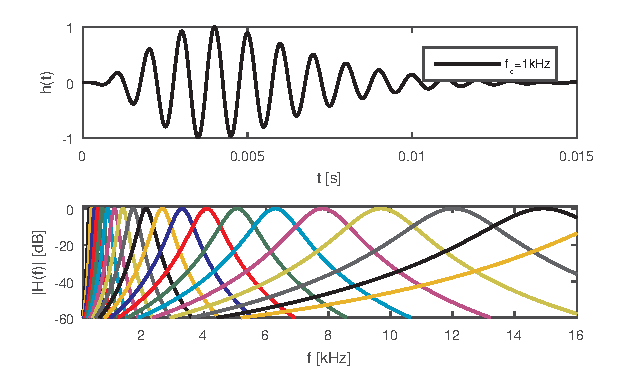
\includegraphics{Gammatone}
                \label{fig:gammatone}
            \end{figure}
        \end{frame}	

    \section[summary]{lecture summary}
        \begin{frame}{summary}{lecture content}
            \begin{enumerate}
                \item       how does the hop length relate to the overlap between blocks?
                \smallskip
                \item<2->   discuss the differences between convolution and correlation in both time and frequency domain
                \smallskip
                \item<3->   name 2 pairs of signals: 
                    \begin{itemize}
                        \item   the correlation function between the signals equals the output of their convolution
                        \item   the correlation function between the signals and the output of their convolution is different.
                    \end{itemize}
                \smallskip
                \item<4->   name 3 important properties of the Fourier transform
                \smallskip
                \item<5->   why are time-frequency transforms helpful tools for audio signal analysis
                \smallskip
                \item<6->   discuss advantages and disadvantages of different approaches for time-frequency transforms
            \end{enumerate}
        \end{frame}
\end{document}

